% Use only LaTeX2e, calling the article.cls class and 12-point type.

\documentclass[12pt,a4paper,english,italian,hidelinks]{article}
\usepackage{fancyhdr}
\usepackage{multirow}
\usepackage{multicol}
\usepackage[section]{placeins}

% === Impostazione dei font ===============================
\usepackage[T1]{fontenc}
\usepackage[utf8]{inputenc}
\usepackage[italian]{babel}
\usepackage{ae}
\usepackage{relsize}
\usepackage{csquotes} 
\usepackage{amsmath}
\usepackage{amsfonts}
\usepackage{mathdots}
\usepackage[colorlinks=true]{hyperref}
\hypersetup{
	bookmarksnumbered=true,
	linkcolor=black,
	citecolor=black,
	pagecolor=black,
	urlcolor=black,
}
\usepackage{verbatim}
\usepackage{alltt}

% Users of the {thebibliography} environment or BibTeX should use the
% scicite.sty package, downloadable from *Science* at
% www.sciencemag.org/about/authors/prep/TeX_help/ .
% This package should properly format in-text
% reference calls and reference-list numbers.

\usepackage{scicite}

% Use times if you have the font installed; otherwise, comment out the
% following line.

\usepackage{times}

% The preamble here sets up a lot of new/revised commands and
% environments.  It's annoying, but please do *not* try to strip these
% out into a separate .sty file (which could lead to the loss of some
% information when we convert the file to other formats).  Instead, keep
% them in the preamble of your main LaTeX source file.

% The following parameters seem to provide a reasonable page setup.

\topmargin 0.0cm
\oddsidemargin 0.2cm
\textwidth 16cm 
\textheight 21cm
\footskip 1.0cm

%The next command sets up an environment for the abstract to your paper.

\newenvironment{sciabstract}{%
\begin{quote} \bf}
{\end{quote}}

% If your reference list includes text notes as well as references,
% include the following line; otherwise, comment it out.

\renewcommand\refname{References and Notes}

% The following lines set up an environment for the last note in the
% reference list, which commonly includes acknowledgments of funding,
% help, etc.  It's intended for users of BibTeX or the {thebibliography}
% environment.  Users who are hand-coding their references at the end
% using a list environment such as {enumerate} can simply add another
% item at the end, and it will be numbered automatically.

\newcounter{lastnote}
\newenvironment{scilastnote}{%
\setcounter{lastnote}{\value{enumiv}}%
\addtocounter{lastnote}{+1}%
\begin{list}%
{\arabic{lastnote}.}
{\setlength{\leftmargin}{.22in}}
{\setlength{\labelsep}{.5em}}}
{\end{list}}

% Include your paper's title here

\title{Mobile Robot} 

% Place the author information here.  Please hand-code the contact
% information and notecalls; do *not* use \footnote commands.  Let the
% author contact information appear immediately below the author names
% as shown.  We would also prefer that you don't change the type-size
% settings shown here.

\author
{Francesco Argentieri	\footnote{ID: 183892 mail: francesco.argentieri@studenti.unitn.it}, 
 Alessandro Luchetti	\footnote{ID: 111111 mail: @studenti.unitn.it},
 Luca Nicolodi				\footnote{ID: 111111 mail: @studenti.unitn.it}\\
\\
\normalsize{Università Degli Studi di Trento, Dipartimento Ingegneria Industriale}\\
\normalsize{C.D.L.M Ingegneria Meccatronica}\\
\normalsize{Corso di Informatica e Programmazione}
}

% Include the date command, but leave its argument blank.

\date{}

% === Integrazione delle figure ===========================
\usepackage{graphicx}
\graphicspath{{./imgs/}}
\renewcommand{\figurename}{Fig.}
\usepackage{subfig}

% === Per gli algoritmi ===================================
\usepackage{algorithmicx}
\usepackage[ruled]{algorithm}
\usepackage{algpseudocode}

% === Per le tabelle ======================================
\usepackage{tabularx}

% === Per la bibliografia multicolonna ====================
\usepackage{etoolbox}
\patchcmd{\thebibliography}{\list}{\begin{multicols}{2}\smaller\list}{}{}
\appto{\endthebibliography}{\end{multicols}}
%==Per le figure latex======================================
%Package e librerie per TikZ e PGF, le librerie non sono tutte necessarie a questo documento LATEX.
\usepackage{tikz, fp, ifthen, fullpage}
     \usepackage{pgfmath}
     \usetikzlibrary{backgrounds}
     \usetikzlibrary{decorations.pathmorphing, backgrounds, fit, calc, through}
     \usetikzlibrary{arrows,chains,matrix,scopes}
     \usetikzlibrary{automata}
     \usetikzlibrary{shapes,decorations,shadows}
     \usetikzlibrary{fadings}
     \usetikzlibrary{patterns}
     \usetikzlibrary{mindmap}
     \usetikzlibrary{decorations.text}
     \usetikzlibrary{decorations.shapes}
      \usepackage{pgfplots}
\pgfplotsset{compat=1.13}

%%%%%%%%%%%%%%%%% END OF PREAMBLE %%%%%%%%%%%%%%%%

\begin{document} 
% Double-space the manuscript.

\baselineskip24pt

% Make the title.

\maketitle 

%===inizio capitoli=================================================

	\section*{Abstract}
Nel report si espongono i risultati raggiunti nello sviluppo del progetto \emph{Mobile Robot}, un robot mobile con azionamento differenziale a due ruote che presenta queste caratteristiche di base:
 LineFollower;
 Riconoscimento incroci nel tracciato;
Comandi da remoto.
Si è scelto di implementarne il funzionamento mediante \emph{macchina a stati finiti}.

%Details for the Course Project Report: The report should be organized with the following sections: 
%TITLE Names and Surnames of the group's components 
%ABSTRACT 
%DESCRIPTION OF THE PROBLEM 
%SOLUTION FOUND Describe the used algorithm/algorithms 
%CONCLUSIONS 
%BIBLIOGRAPHY 
%The maximum allowed number of pages is 6, every page that exceed this limit will be ignored. Pictures, chart and plots can be added to the report.

	%%%%%%%%%%%%%%%%%%%%%%%%%%%%%%%%%%%%%%%%%%%%%%%%%%%%%%%%%%%

\chapter{Introduzione}
\label{chap:Introduzione}

%%%%%%%%%%%%%%%%%%%%%%%%%%%%%%%%%%%%%%%%%%%%%%%%%%%%%%%%%%%

\section{Contesto applicativo}
\label{sec:intro1}

Ciao ragazzi :D questo è un template che potete utilizzare per scrivere la vostra tesi in \LaTeX (sì, il nome di questo linguaggio è tutto un programma...)

Cos'è \LaTeX ? Cercatevelo su Wikipedia\footnote{http://it.wikipedia.org/wiki/LaTeX}!

A parte gli scherzi... è un linguaggio che vi permette (in poche parole) di creare documenti accademici (e non) con uno stile molto professionale. Gran parte del lavoro sporco (creazione dei capitoli, delle sezioni, dell'indice, della bibliografia, gestione dei margini, ecc...) viene interamente gestito da \LaTeX , le poche cose da configurare sono già state impostate in questo template... (quindi in poche parole avete già tutto pronto, stronzi!)

In questo pdf è spiegato un po' come far funzionare il tutto, ovvero:
\begin{itemize}
\item Dove scaricare l'IDE e come configurarlo
\item Come scaricare il compilatore
\item Come iniziare a personalizzare questo template
\end{itemize}

Cercherò di utilizzare più elementi \LaTeX possibile nello scrivere questa guida (tabelle, elenchi puntati, footnote, immagini...) così quando andrete a leggere il codice vi imparate pure qualcosa, caproni (<3)

%%%%%%%%%%%%%%%%%%%%%%%%%%%%%%%%%%%%%%%%%%%%%%%%%%%%%%%%%%%

\section{Motivazioni e obiettivi}
\label{sec:intro2}

Il principale motivo che mi spinge a creare questo pdf è quello di risparmiarvi gran parte delle rotture che si trovano quando ci si avvicina al mondo \LaTeX... insomma mi auguro che questa guida vi permetta di avere un buon punto d'inizio.

Come già spiegato nella sezione precedente, \LaTeX offre tantissimi servizi utili ed uno stile professionale unico, cose che su altri programmi (come Microsoft Word) potete anche sognarvi.

Insomma... con \LaTeX potete presentare una tesi fatta come si deve :)

%%%%%%%%%%%%%%%%%%%%%%%%%%%%%%%%%%%%%%%%%%%%%%%%%%%%%%%%%%%

\section{Risultati raggiunti}
\label{sec:intro3}

Nella Figura \ref{fig:latexVsWord} potete ammirare quanto \LaTeX sia più figo di Microsoft Word, ooooooh...

\begin{figure}[h] %La "h" indica che la figura si posizionerà "here". Usate "t" per "top" e "b" per "bottom"
\centering %centrata
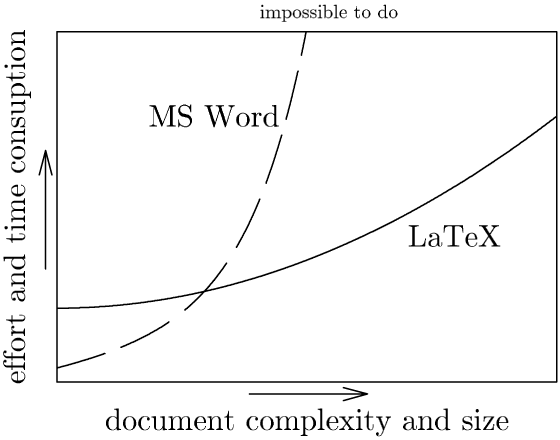
\includegraphics[width=0.8\linewidth]{latexVsWord} %larghezza e nome del file
\caption{Oooooooh che figo \LaTeX, ooooooooh} %didascalia
\label{fig:latexVsWord} %label per il riferimento
\end{figure}

%%%%%%%%%%%%%%%%%%%%%%%%%%%%%%%%%%%%%%%%%%%%%%%%%%%%%%%%%%%

\section{Organizzazione della tesi}
\label{sec:intro4}

Vi spiego brevemente quali sono le parti di questo template:

\begin{description}
  \item[Susanna.tex] Questo è il file principale del template: contiene le impostazioni generali e la struttura della tesi. Ricordate di impostarlo come documento master ogni volta che iniziate a lavorare alla tesi (ovviamente potete rinominarlo, nabbazzi)
  \item[frontespizio.tex] Sarebbe la copertina della tesi, nonchè la prima pagina. Contiene nome dell'università, del dipartimento, nome della tesi bla bla bla... io ho scelto un argomento di Fisica molto importante <3
  \item[dedica.tex] Una pagina dove scrivete a chi dedicate la tesi (Susanna <3)
  \item[introduzione.tex] Il file che contiene questo capitolo introduttivo (vi consiglio di creare appunto un file .tex per ogni capitolo). Le 4 sezioni di questo capitolo (\nameref{sec:intro1}, \nameref{sec:intro2}, \nameref{sec:intro3} e \nameref{sec:intro4}) sono le 4 sezioni standard da inserire nell'introduzione di una tesi, quindi vi consiglio di lasciarle così
  \item[start.tex] Contiene l'unico capitolo utile di questo documento: spiega come scaricare l'occorrente e come configurare il tutto per lavorare con \LaTeX
  \item[conclusione.tex] Contiene la conclusione (YOU DON'T SAY)
  \item[bibliografia.bib] Contiene i dati relativi alle fonti che citerete nella tesi (ad esempio, ora sto citando un libro sugli algoritmi genetici \cite{5635176}, l'unico inserito nella bibliografia di questo template)
  \item[IEEEtran.bst] È lo stile della bibliografia, non lo toccate
  \item[imgs] Cartella contenente le immagini (YOU DON'T SAY AGAIN)
\end{description}


	\section{Soluzione del problema}
\label{solution}
Nel dettaglio si descrive il software del robot partendo dallo strato che interfaccia le periferiche con l'unità di elaborazione.
\subsection{Libreria Makeblock}
L'utilizzo di questa libreria è stato fondamentale perché rappresenta la base dei tre livelli e permette allo sviluppatore di istanziare i moduli fisici come oggetti e di renderli operativi fin da subito dato che viene richiesta solo la porta a cui sono collegati.
Utilizzando i metodi disponibili dalla classe è possibile ricavare gli input provenienti dai sensori, permettere la comunicazione con altri dispositivi mediante bluetooth, pilotare i motori.
\subsection{Libreria Macchina a stati finiti}
Questo secondo strato software è stato sviluppato durante le esercitazioni di laboratorio.

\begin{figure}[h!t]
\centering
\subfloat[][\emph{Schema concettuale}.]
   {\begin{tikzpicture}[->, >=stealth', shorten >=1pt, auto, node distance=2.5cm, semithick]

%====Definizione stile stati================================================

	\tikzstyle{every state}=[fill, draw=none, orange ,text=white]
  	\tikzstyle{accepting}=[green!50!black, text=white]
  	\tikzstyle{initial}= [red, text=white]

%====Definizione stati e posizione===========================================
	\node[state,initial] 			(A)                    		{\textsc{A}};
 	\node[state]          			(B) [right of=A]		{\textsc{B}};
 	\node[state,accepting]	(C) [right of=B]		{\textsc{C}};
  	\node[state]         			(D) [right of=C]  		{\textsc{D}};
  	
%====Definizione collegamenti e stile frecce================================================================
      			 %from     stile                      scritte       	to		
      \path 	(A)		edge	[right]									(B)
      				(B)		edge	[bend left]							(C)
      				(C)		edge	[bend left]							(B)
      				(C)		edge[right]									(D)
      				(D)		edge[bend left]							(A);    
\end{tikzpicture}} \qquad\quad
\subfloat[][\emph{Legenda}.]{\begin{tikzpicture}[->, >=stealth', shorten >=1pt, auto, node distance=1.5cm, semithick]

%====Definizione stile stati================================================

	\tikzstyle{every state}=[fill, draw=none, orange ,text=white]
  	\tikzstyle{accepting}=[green!50!black, text=white]
  	\tikzstyle{initial}= [red, text=white]

%====Definizione stati e posizione===========================================

	\node[state,initial] 			(A) [label = 0:Init ]                  		{\textsc{A}}; 	
 	\node[state]          			(B) [below of= A, label = 0:Start]		{\textsc{B}};		
 	\node[state,accepting]	(C) [below of= B, label = 0:Line Follower]		{\textsc{C}};
  	\node[state]         			(D) [below of= C, label = 0:Manual Control]  		{\textsc{D}};		

%====Definizione collegamenti e stile frecce================================================================
      			 %from     stile                      scritte       	to		
%      \path 	(A)		edge	[right]									(B)
%      				(B)		edge	[bend left]						(C)
%      				(C)		edge	[bend left]						(B)
%      				(C)		edge[right]								(D)
%      				(D)		edge[bend left]						(A);    
\end{tikzpicture}}
\caption{Macchina a stati finiti}
\label{msf}
\end{figure}

\subsection{Libreria}
Infine questa libreria gestisce la risposta del robot al variare degli input durante il suo funzionamento, rappresenta lo strato di interconnessione tra i due prima analizzati.
Questa classe inizializza un oggetto che ammette in input i dati provenienti del sensore a ultra suoni e dai sensori di linea: con il primo dato verifica la presenza di ostacoli nella parte frontale se assenti o distanti almeno $15 \, cm$ da il via libera a proseguire lungo a direzione altrimenti impartisce al robot il comando di ruotare sul proprio asse e proseguire nella direzione opposta.
Con il secondo input proveniente dai sensori di linea riconosce il percorso affrontato secondo una serie di casi codificati secondo la tabella \ref{error_normali} attribuendo un errore. Tale valore viene utilizzato per corregere la velocità dei motori tramite un controller \textsc{pd}, si descriverà in dettaglio nella sezione \ref{PID}.
Vengono inoltre codificati dei casi eccezionali consultabili nella tabella \ref{eccezioni} a cui è stato assegnato un errore $0$ perchè \dots

\begin{table}[h]
\center
\begin{tabular}{llccr}
\label{normali}
                             %      (X=nero; O=bianco)
                          			&			&DX  SX&	SX  DX    	& Errore\\
\hline \\
  GO FORWARD          		& ==  	&1, 2  	& O X  X O 	& 0\\				% (line = nero & background = bianco) 
  TURN LEFT VERY SOFT 	&	==	&	3, 2	&	O X  O O  &	1\\
  TURN LEFT SOFT       	&	==  	&	1,	0	&	X X  X O   &	2\\
  TURN LEFT HARD     		&	==  	&	3, 0	&	X X  O O	&	3\\
  TURN LEFT VERYHARD  &	==  	&	3, 1	&	X O  O O	&	4\\
  TURN RIGHT VERY SOFT&	== 	& 1, 3	&	O O  X O  &	-1\\
  TURN RIGHT SOFT    		&	==  	&	0, 2	& 	O X  X X  	&	-2\\
  TURN RIGHT HARD   		&	== 	&	0, 3	&	O O  X X  	&	-3\\
  TURN RIGHT VERYHARD &	== 	&	2, 3	&	O O  O X	&	-4\\
  NO LINE           				&	== 	&	3, 3	&	O O  O O  &	  5\\
  CROSS              				&	== 	& 0, 0   &	X X  X X   	&  6\\\\
  \hline
\end{tabular}
\caption{Codifica input dei sensori di linea (X = tracciato nero; O = sfondo bianco)}
\label{error_normali}
\end{table}

\begin{table}
\center
\begin{tabular}{llccc}
\label{eccezioni}
								&			&	DX  SX	&	SX  	DX    &    Errore\\
 \hline\\
	GO FORWARD bis    	&	== 	&	2, 1		&	X O  O X	&  0\\
	EXCEPTION1       		&	==  	&	2, 0		&	X X  O X   &	0\\
  	EXCEPTION2        	&	== 	&	0, 1  	&	X O  X X   &  0\\
 	EXCEPTION3     	 	&	==  	&	2, 2	 	&	O X  O X	&  0\\\\
  \hline
\end{tabular}
\caption{Codifica \textsc{casi eccezionali} (X = tracciato nero; O = sfondo bianco)}
\label{eccezioni}
\end{table}

\noindent Quando il robot raggiunge un incrocio si arresta uscendo dallo stato di line follower e passa nello stato idle attendendo istruzioni dall'utente che può scegliere dalla maschera disponibile sul terminale, quindi inviare il comando tramite connessione bluetooth. Il robot torna nello stato di linefollower.

%Il modo più efficiente di progettare un controllo di un robot di questo tipo è basato sul modello di macchina a stati finiti in cui ad ogni stato corrisponde una specifica funzione del robot.
%% inserire diagramma a stati e riferimento alla figura
%Lo stato è  caratterizzato da una funzione d'ingresso (\emph{enter function}), una funzione di aggiornamento (\emph{update function}), un funziona di uscita (\emph{exit function}).
%La transizione da uno stato all'altro è soggetta al soddisfacimento di una certa condizione.


%\subsection{Stato Init}
%Stato di inizializzazione della macchina all'avvio del robot. Garantisce lo stato di fermo dei motori mediante il richiamo della funzione di stop e poi si aggiorna con la funzione start che  invoca la transizione verso lo \emph{stato Idle}.
%
%\begin{figure}[htb]
%\centering
%\subfloat[][\emph{Stato}.]{\begin{tikzpicture}[->, >=stealth', shorten >=1pt, auto, node distance=2.5cm, semithick]
%%====Definizione colori 	 paticolari===========================================
%	\definecolor{royalblue}{cmyk}{1,0.50,0,0}
%  	\definecolor{cerulean}{cmyk}{0.94,0.11,0,0}
%	\definecolor{violet}{cmyk}{0.79,0.88,0,0}
%%====Definizione stile stati================================================
%	\tikzstyle {state1}=[circle, top color=white, bottom color=orange!40, draw, violet, minimum width=1cm]
%	\tikzstyle{state2}=[circle, top color=white, bottom color=cerulean!40, draw, royalblue, minimum width=1cm]
%%====Definizione stati e posizione===========================================
%	%\draw[very thick] (2.5,0)circle[radius=4cm];
%	\draw [very thick,dashed](2.5,0) ellipse (4.5cm and 2cm);
%	\node[state1]	(A)          			{$f_{1}$};
% 	\node[state2]	(B) [right of=A]	{$f_{2}$};
% 	\node[state1]	(C) [right of=B]	{$f_{3}$};
%%====Definizione collegamenti e stile frecce================================================================
%      			 %from     stile                      scritte       	to		
%      \path 	(A)		edge	[bend left]							(B)
%      				(B)		edge	[bend left]							(C)
%      				(C)		edge	[bend left]							(B)
%	     			(B)		edge	[bend left]							(A);   
%\end{tikzpicture}}\qquad\quad
%\subfloat[][\emph{Legenda}.]{\begin{tikzpicture}[->, >=stealth', shorten >=1pt, auto, node distance=1.5cm, semithick]
%%====Definizione colori 	 paticolari===========================================
%	\definecolor{royalblue}{cmyk}{1,0.50,0,0}
%  	\definecolor{cerulean}{cmyk}{0.94,0.11,0,0}
%	\definecolor{violet}{cmyk}{0.79,0.88,0,0}
%%====Definizione stile stati================================================
%	\tikzstyle {state1}=[circle, top color=white, bottom color=orange!40, draw, violet, minimum width=1cm]
%	\tikzstyle{state2}=[circle, top color=white, bottom color=cerulean!40, draw, royalblue, minimum width=1cm]
%%====Definizione stati e posizione===========================================
%	\node[state1]	(A) [label = 0: \textsc{enter function}]           			{$f_{1}$};
% 	\node[state2]	(B) [below of=A, label = 0:\textsc{update function}]	{$f_{2}$};
% 	\node[state1]	(C) [below of=B, label = 0:\textsc{update function}]	{$f_{3}$}; 
%\end{tikzpicture}}
%\caption{Rappresentazione interna dello stato}
%\label{stato}
%\end{figure}
%
%
%\subsection{Stato Idle}
%In questo stato l'enter function richiama la funzione che stampa sul terminale i comandi disponibili per l'interazione con l'utente, poi passa nell'update function  che aspetta il comando dell'utente inviato tramite il bluetooth per la transizione nello stato successivo.

%\subsection{Stato Line Follower}
%Nel seguente stato la prima operazione che viene eseguita è una lettura mediante sensore ad ultrasuoni della presenza di eventuali ostocali sul tracciato.
%La distanza di sicurezza scelta sperimentalmente è di $15 \, cm$ valore che permette al robot di arrestarsi e ruotare su stesso evitando contatti con l'ostacolo.
%Verificata tale condizione inizia la lettura dei sensori di linea che decifrano il percorso secondo la logica presentata in tabella \ref{error_normali}. Casi eccezionali in tabella \ref{eccezioni}. Ad ogni casistica è stato associato un errore che attraverso un controllo PD appositamente 
%implementato fornisce il valore di correzione da inviare ai motori per rimanere sul tracciato.

%FUNZIONE %path_error
%  in questa funzione in ingresso vengono ricevuti
%  due interi ricavati dai metodi dei line follewer
%  e in uscita viene restituito un intero che individua la posizione del 
%  robot rispetto alla linea da seguire (error = output - setpoint).
%  Sulla base dei valori ricevuti dai sensori si ottengono i seguenti casi:\\
%\subsection{Stato Manual Command}
	\section{Controller PID}
\label{PID}

\begin{figure}[htb]
\centering
\label{PIDimage}
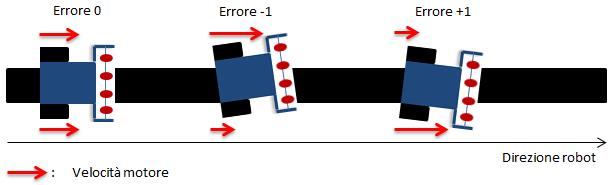
\includegraphics[width=0.65 \textwidth]{PID.jpg} 
\caption{prova}
\end{figure}

\begin{figure}[htb]
\centering
\label{PD}
\begin{tikzpicture}[->, >=stealth', shorten >=0.1pt, auto, node distance=2cm, semithick,
								  hv path/.style={to path={-| (\tikztotarget)}},
								  tip/.style={->,shorten >=0.007pt}, 
								  vh path/.style={to path={|- (\tikztotarget)}}]

%====Definizione stile stati===============================================

	\tikzstyle{sommatore} = [circle, draw, text centered,  minimum width =0.02cm]
  	\tikzstyle{block}			=	[rectangle, draw, text centered, minimum height =1cm]
  	\tikzstyle{line} = [, draw]
%====Definizione stati e posizione==========================================
	\node[] 					(A) [label = set point]                   		{};
	\node[sommatore]  (B) [right of=A, node distance = 3cm, label = -240:$+$,label = -120:$-$]		{$\sum$};			
	\node[block]			(C) [right of=B, node distance = 3cm ]		{\textsc{pd}};
  	\node[sommatore] 	(D) [right of=C,node distance = 	3cm 	]		{} ;
  	\node[]         			(E) [right of=D,node distance = 	3cm, label = 90:uscita, label =- 90: velocita motori]  		{};
 	\node[]         			(F) [below of=B]  	{};
  	\node[]         			(G) [below of=D]  	{};
  	\node[block]         	(H) [below of=C]  	{\textsc{sensori di linea}}; 	
%====Definizione chain==================================================
    
       \path	 	(A) edge (B)
        			 	(B) edge node{errore}(C)
        				(C) edge (D);
        { [start chain]
        \chainin	(D) [join];
        { [start branch=minus]
        	\chainin (H) [join=by {vh path,tip}];
        	\chainin (B) [join=by {hv path,tip}];
        }
		\chainin(E) [join];				
    }				
\end{tikzpicture}
\caption{prova}
\end{figure}

	\section{Conclusione}
\label{conclusione}
Lo sviluppo del software ha permesso di soddisfare le richieste di line following infatti il robot riesce autonomamente ad adattarsi a diversi tipi di tracciato e muoversi anche nei casi più difficili. Il setup utilizzato nel controllore \textsc{PID} permette di spingere il robot al $55\%$ della velocità massima consentita dai motori senza incorrere in slittamenti o sbandate. Permette all'utente di interagirvi con la possibilità di scegliere la direzione di svolta nel caso di incrocio e pilotarlo da remoto tramite conessione bluetooth. Infine in tutti i casi il robot evita autonomamente l'impatto con gli ostacoli.
	%
\begin{tikzpicture}[->, >=stealth', shorten >=1pt, auto, node distance=2.8cm, semithick]
%====Definizione colori 	 paticolari===============================================================
	\definecolor{royalblue}{cmyk}{1,0.50,0,0}
  	\definecolor{cerulean}{cmyk}{0.94,0.11,0,0}
	\definecolor{violet}{cmyk}{0.79,0.88,0,0}
%====Definizione stile stati===============================================================
	\tikzstyle {state1}=[circle, top color=white, bottom color=orange!40, draw, violet, minimum width=1cm]
	\tikzstyle{state2}=[circle, top color=white, bottom color=cerulean!40, draw, royalblue, minimum width=1cm]
%  \node[initial,state] (A)                    {$init$};
%  \node[state]         (B) [above right of=A] {$idle$};
%  \node[state]         (D) [below right of=A]  {$line follower$};
%  \node[state]         (C) [below right of=B]  {$stop$};
%  \node[state]         (E) [below of=D]        {$q_e$};
%  \node[state]			(F)[ right of=B]{$start$};
%====Definizione stati e posizione===============================================================
	\node[initial,state1] 	(A)                    		{$init$};
 	\node[state2]          	(B) [right of=A]		{$START$};
 	\node[state1]		   		(C) [right of=B]		{$IDLE$};
  	\node[state2]         	(D) [right of=C]  		{$line follower$};
  	\node[state1]          	(E) [below of=C]  	{$stop$};
%  \path (A) 	edge             			 node {0,1,L} (B)
%            		edge              			node {1,1,R} (C)
%        	(B) 	edge [loop above] 	node {1,1,L} (B)
%            		edge              			node {0,1,L} (C)
%        	(C)	 edge              			node {0,1,L} (D)
%            		edge [bend left]  		node {1,0,R} (E)
%        	(D) 	edge [loop below] 	node {1,1,R} (D)
%            		edge              			node {0,1,R} (A)
%       		(E) 	edge [bend left]  		node {1,0,R} (A)
%       		(F)	edge												 (D);
%====Definizione collegamenti e stile frecce===============================================================
      			 %from     stile                      scritte       	to		
      \path 	(A)		edge	[right]									(B)
      				(B)		edge												(C)
      				(C)		edge												(D)
      				(D)		edge	[bend left]							(E)
      				(D)		edge[bend right]							(C)
      				(E)		edge[bend left]							(C);    
\end{tikzpicture}



    
\begin{tikzpicture}[->, >=stealth', shorten >=1pt, auto, node distance=2.8cm, semithick]
 % Define block styles
	\tikzstyle{decision} = [diamond, draw, fill=blue!20, text width=4.5em, text badly centered, node distance=3cm, inner sep=0pt]
\tikzstyle{block} = [rectangle, draw, fill=blue!20, text width=5em, text centered, rounded corners,  minimum height=4em]
%	\tikzstyle{line} = [draw, -latex']
	\tikzstyle{input/output} =[trapezium, draw, minimum width=3cm,
trapezium left angle=60, trapezium right angle=120]
	\tikzstyle{start/stop} = [draw, ellipse,fill=red!20, node distance=3cm, minimum height=2em]
%%====Definizione stati e posizione===============================================================
	\node	[start/stop]		(start)										{start};
	\node	[input/output]	(sensori)	[below of= start]		{prova};
    \node 	[block] (init) 					[below of= sensori]	{initialize model};
    \node	[block]	(test)					[below of= init]		{daje};
    \node	[]()[]{};
%   \node [cloud, left of=init] (expert) {expert};
%    \node [cloud, right of=init] (system) {system};
%    \node [block, below of=init] (identify) {identify candidate models};
%    \node [block, below of=identify] (evaluate) {evaluate candidate models};
%    \node [block, left of=evaluate, node distance=3cm] (update) {update model};
%    \node [decision, below of=evaluate] (decide) {is best candidate better?};
%    \node [block, below of=decide, node distance=3cm] (stop) {stop};
%    % Draw edges
%    \path [line] (init) -- (identify);
%    \path [line] (identify) -- (evaluate);
%    \path [line] (evaluate) -- (decide);
%    \path [line] (decide) -| node [near start] {yes} (update);
%    \path [line] (update) |- (identify);
%    \path [line] (decide) -- node {no}(stop);
%    \path [line,dashed] (expert) -- (init);
%    \path [line,dashed] (system) -- (init);
%    \path [line,dashed] (system) |- (evaluate);
\end{tikzpicture}


%===bibliografia=================================================
\nocite{*}
\bibliography{scibib}

\bibliographystyle{Science}

% Following is a new environment, {scilastnote}, that's defined in the
% preamble and that allows authors to add a reference at the end of the
% list that's not signaled in the text; such references are used in
% *Science* for acknowledgments of funding, help, etc.

% For your review copy (i.e., the file you initially send in for
% evaluation), you can use the {figure} environment and the
% \includegraphics command to stream your figures into the text, placing
% all figures at the end.  For the final, revised manuscript for
% acceptance and production, however, PostScript or other graphics
% should not be streamed into your compliled file.  Instead, set
% captions as simple paragraphs (with a \noindent tag), setting them
% off from the rest of the text with a \clearpage as shown  below, and
% submit figures as separate files according to the Art Department's
% instructions.

\clearpage
\end{document}
